% !TeX spellcheck = en_US
\documentclass[a4paper]{article}
\usepackage[utf8]{inputenc}
\usepackage{t1enc}
\usepackage[english]{babel}
\usepackage{lmodern}
\usepackage{url}
\usepackage{graphics}
\usepackage{listings}
\usepackage[a4paper, total={5.4in, 8in}]{geometry}

\hyphenation{UPPAAL}
\sloppy

\begin{document}
	
	\newcommand{\specialcell}[2][c]{%
		\begin{tabular}[#1]{@{}l@{}}#2\end{tabular}}
	
	\newenvironment*{mytable}[3]{
		% #1: caption, #2: cimke, #3: oszlopdef		 
		\begin{table}[htbp]	
			\caption{#1}          
			\label{tab:#2}            
			\center%
			\begin{tabular}{#3}
			}
			{
			\end{tabular}
		\end{table}
	}
	
	\pagestyle{plain}
	
	
	
	% angol környezet beállítása
	\nonfrenchspacing
	\setlength{\parindent}{0em}
	\setlength{\parskip}{0.45em}
	
	\title{Language Learning Application: \\ Requirement Specification \\ \begin{large}Software Architectures Homework \end{large}}
	\author{Bence Graics \and Kristóf Verbőczy}	
	\date{}
	\maketitle
	\section*{Introduction}
	This document presents the requirement specification of the software architectures homework \textsl{Language Learning Application}. First, the assigned task is introduced, which is followed by the detailed description of the task. Next, the technical parameters of the software developed for the particular task are presented. Additionally, high level requirements for the developed software are described. Finally, a use-case diagram is displayed that depicts the essential use-cases of the software.
	\section{The task}
	The task is to create an application aiding foreign language learning. The foreign words and sentences can be organized into lessons by means of associated meta information. A central server is responsible for the management and storage of data. In addition to a server component, the application comprises of a client component supporting the management of the server as well as the conduction of lessons. The platforms, serving as the basis of the application, can be chosen freely.
	
	\section{Detailed task description}
	The goal of the project is to create an application that facilitates the learning of English language for Hungarian speakers.
	
	To facilitate the use of the application, all functionalities shall be reachable via a graphical interface. The application shall support the registration and authentication of users. The application shall be used only by authenticated users, that is,  users shall be requested to login before any functionality of the application could be utilized. There shall be two types of users: \textsl{simple user} and \textsl{super user}. Both types of users shall be able to use the following functionalities: \emph{learning} the English language via lessons and \emph{creating exercises}. Additionally, super users shall be able to \emph{register new users} and \emph{delete exercises}.
	
	The learning activity shall be conducted based on \emph{lessons}. A lesson shall consist of two phases: a \emph{coaching} period, where the goal is to introduce new English words and phrases to the user, and an \emph{exercising} period, where the acquired knowledge of the user shall be checked. The application shall have three types of exercises:
	\begin{itemize}
		\item choosing the correct Hungarian word for an English word from four possible words,
		\item giving (typing) a correct Hungarian phrase for an English phrase,
		\item giving (typing) a correct Hungarian or English word (according to the task) for an object that is depicted by a figure.
	\end{itemize}
	A single lesson shall comprise of ten exercises which are randomly chosen from a database based on the knowledge level of the playing user. The application shall count the correct answers given by particular users during lessons. On correct answers the application shall give the users \emph{experience points}, which represent the knowledge level of a particular user. Higher level users shall receive harder exercises during lessons. 

	Exercises shall be created in one of the following ways:
	\begin{itemize}
		\item a single English-Hungarian word pair can be registered to the application,
		\item a single English-Hungarian phrase pair can be registered to the application,
		\item a figure depicting an object can be added in addition to the English and Hungarian words that describe the particular object.
	\end{itemize}
	
	
	\section{Requirements}
	This section introduces the mandatory and optional requirements regarding the application.
	\begin{enumerate}
		\item Mandatory: The application shall allow somebody to login only if she typed in an existing user name and the associated password.
		\item Mandatory: A user without super user privileges shall not be able to delete anything from the database.
		\item Mandatory:  The application shall validate the content of input fields given by users.
		\item Mandatory:  The application shall be able to recognize and counter SQL injection attacks.
		\item Mandatory:  The database shall store the hash values of the passwords instead of the plain text.
		\item Mandatory: The application shall allow authenticated users to create new exercises.
		\item Optional: A user with super user privileges shall be able to delete exercises from the database.
		\item Mandatory: The business logic shall provide a coaching phase before the exercising phase.
		\item  Mandatory:  The business logic shall provide exercises matching or below the user's knowledge level.
		\item Optional: The application server shall be able to serve multiple clients parallely. 

	\end{enumerate}
	
	\section{Technical parameters}
	Both the client and server components of the application are going to be based on the Java 8 platform in order to enhance reuse on all platforms. The graphical interface of the application is going to be developed using JavaFX. The server is going to be based on an Oracle relational database version 11.0. The running of the server component is going to be based on Maven WildFly version 1.7.0. The client and server components are going to communicate through REST calls.
	
	\section{Use-cases}
	Figure \ref{fig:use-case} depicts the high level use-cases of the application.
	\begin{figure}[htbp]
		\center
		\resizebox{155mm}{!} {
			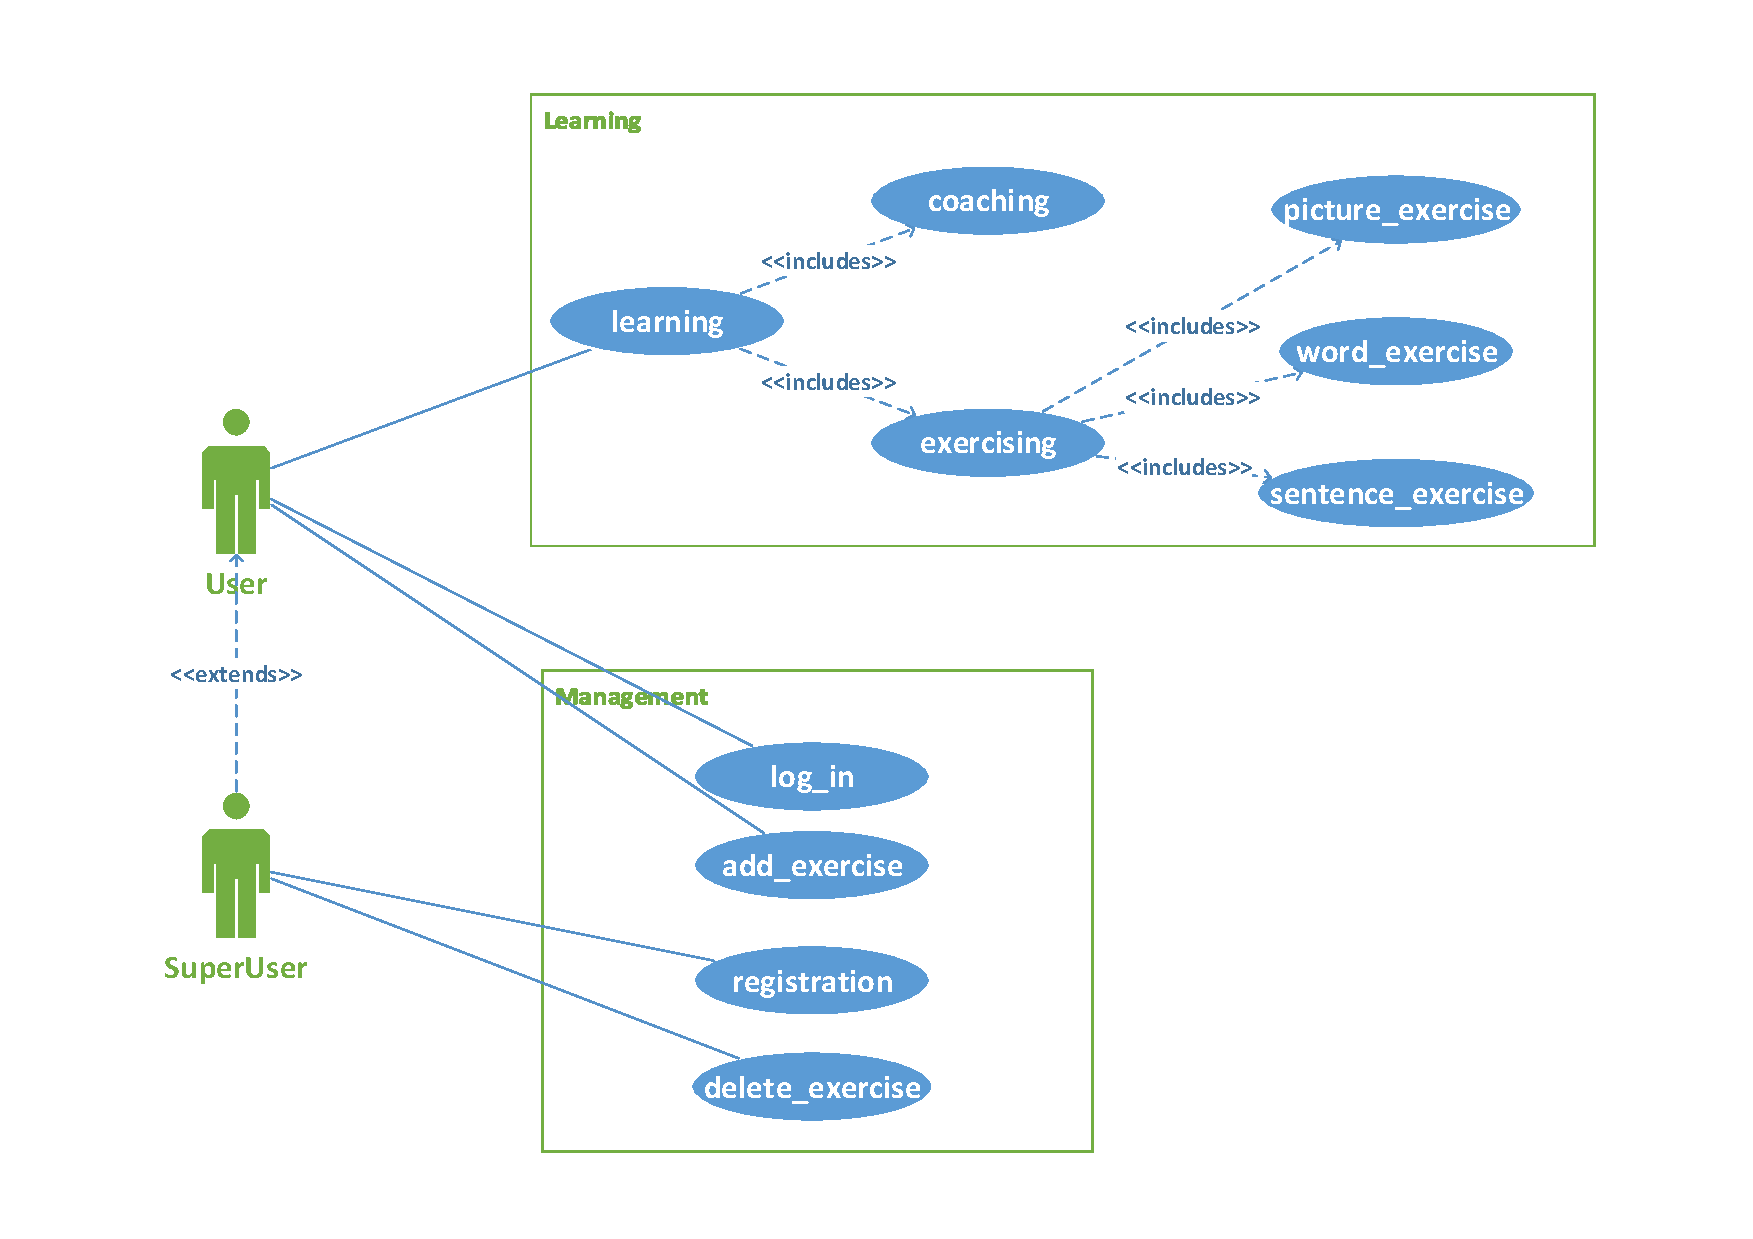
\includegraphics{figures/use-case.pdf}
		}
		\caption{Use-case diagram depicting the use-cases of the application.}
		\label{fig:use-case}
	\end{figure}

\end{document}